% 20131014-135722
% B8.0/W11.0

\section{B8.0/W11.0 - 110 krpm}
\label[secinapp]{sec:bwp-exp-details-B8.0/W11.0}

This test has been performed on October 14\th{} 2013, at 13:57:22,
just before the break of the compression unit.

\begin{table}[htbp]
  \footnotesize
  \begin{center}
    \begin{tabular}{cccccc}
\toprule
Component & Location & P / \si{\bar} & T / \si{\degreeCelsius} & h / \si{\kilo\joule\per\kilo\gram} & s / \si{\kilo\joule\per\kilo\gram\per\kelvin}\\
\midrule
\multirow{2}{*}{1} & inlet & $ \num{2.39} \pm \num{0.03} $ & $ \num{24} \pm \num{7} $ & $ \num{420.822} \pm \num{0.007} $ & $ \num{1.82} \pm \num{0.02} $\\
& outlet & $ \num{3.90} \pm \num{0.03} $ & $ \num{45} \pm \num{7} $ & $ \num{436.899} \pm \num{0.006} $ & $ \num{1.84} \pm \num{0.02} $\\
\midrule
\multirow{2}{*}{2} & inlet & $\pmb{ \num{3.642} \pm \num{0.002} }$ & $\pmb{ \num{36.174} \pm \num{0.007} }$ & $ \num{429.572664} \pm \num{7e-06} $ & $ \num{1.81710} \pm \num{6e-05} $\\
& outlet & $\pmb{ \num{5.110} \pm \num{0.002} }$ & $\pmb{ \num{50.73} \pm \num{0.01} }$ & $ \num{440.61999} \pm \num{1e-05} $ & $ \num{1.82642} \pm \num{6e-05} $\\
\midrule
\multirow{2}{*}{3} & inlet & $\pmb{ \num{4.954} \pm \num{0.002} }$ & $\pmb{ \num{49.45} \pm \num{0.01} }$ & $ \num{439.66514} \pm \num{1e-05} $ & $ \num{1.82580} \pm \num{6e-05} $\\
& outlet & $\pmb{ \num{4.776} \pm \num{0.002} }$ & $\pmb{ \num{10.91} \pm \num{0.01} }$ & $ \num{214.83703} \pm \num{1e-05} $ & $ \num{1.05274} \pm \num{5e-05} $\\
\midrule
\multirow{2}{*}{4} & inlet & $ \num{2.60} \pm \num{0.03} $ & $ \num{-3.2} \pm \num{0.3} $ & $ \num{223.8405} \pm \num{3e-04} $ & $ \num{1.089} \pm \num{0.001} $\\
& outlet & $\pmb{ \num{2.603} \pm \num{0.002} }$ & $\pmb{ \num{7.53} \pm \num{0.01} }$ & $ \num{406.14017} \pm \num{1e-05} $ & $ \num{1.7631} \pm \num{1e-04} $\\
\midrule
\multirow{2}{*}{5} & inlet & $ \num{4.78} \pm \num{0.03} $ & $ \num{10.91} \pm \num{0.03} $ & $ \num{214.83703} \pm \num{3e-05} $ & $ \num{1.0527} \pm \num{1e-04} $\\
& outlet & $ \num{3.77} \pm \num{0.02} $ & $ \num{7.2} \pm \num{0.2} $ & $ \num{214.8370} \pm \num{2e-04} $ & $ \num{1.0531} \pm \num{8e-04} $\\
\midrule
\multirow{2}{*}{6} & inlet & $ \num{3.77} \pm \num{0.02} $ & $ \num{7.2} \pm \num{0.2} $ & $ \num{214.8370} \pm \num{2e-04} $ & $ \num{1.0531} \pm \num{8e-04} $\\
& outlet & $ \num{2.60} \pm \num{0.03} $ & $ \num{-3.2} \pm \num{0.3} $ & $ \num{214.8370} \pm \num{3e-04} $ & $ \num{1.055} \pm \num{0.001} $\\
\midrule
\multirow{2}{*}{7} & inlet & $ \num{4.78} \pm \num{0.03} $ & $ \num{10.91} \pm \num{0.03} $ & $ \num{214.83703} \pm \num{3e-05} $ & $ \num{1.0527} \pm \num{1e-04} $\\
& outlet & $ \num{2.60} \pm \num{0.03} $ & $ \num{-3.2} \pm \num{0.3} $ & $ \num{243.3710} \pm \num{3e-04} $ & $ \num{1.161} \pm \num{0.001} $\\
\midrule
\multirow{2}{*}{8} & inlet & $ \num{5.11} \pm \num{0.03} $ & $ \num{50.7} \pm \num{0.2} $ & $ \num{440.6200} \pm \num{1e-04} $ & $ \num{1.8264} \pm \num{7e-04} $\\
& outlet & $ \num{2.39} \pm \num{0.03} $ & $ \num{46.0} \pm \num{0.2} $ & $ \num{440.6200} \pm \num{1e-04} $ & $ \num{1.885} \pm \num{0.001} $\\
\midrule
\multirow{2}{*}{9} & inlet & $ \num{3.77} \pm \num{0.02} $ & $ \num{7.2} \pm \num{0.2} $ & $ \num{214.8370} \pm \num{2e-04} $ & $ \num{1.0531} \pm \num{8e-04} $\\
& outlet & $ \num{3.77} \pm \num{0.02} $ & $ \num{7.2} \pm \num{0.2} $ & $ \num{214.8370} \pm \num{2e-04} $ & $ \num{1.0531} \pm \num{8e-04} $\\
\midrule
\multirow{2}{*}{10} & inlet & $ \num{5.11} \pm \num{0.03} $ & $ \num{50.7} \pm \num{0.2} $ & $ \num{440.6200} \pm \num{1e-04} $ & $ \num{1.8264} \pm \num{7e-04} $\\
& outlet & $ \num{3.90} \pm \num{0.03} $ & $ \num{51} \pm \num{8} $ & $ \num{442.593} \pm \num{0.007} $ & $ \num{1.85} \pm \num{0.02} $\\
\midrule
\multirow{2}{*}{11} & inlet & $ \num{3.19} \pm \num{0.03} $ & $ \num{8.0} \pm \num{0.3} $ & $ \num{405.0528} \pm \num{2e-04} $ & $ \num{1.744} \pm \num{0.001} $\\
& outlet & $ \num{3.19} \pm \num{0.03} $ & $ \num{12} \pm \num{10} $ & $ \num{408.87} \pm \num{0.01} $ & $ \num{1.76} \pm \num{0.03} $\\
\midrule
\multirow{2}{*}{12} & inlet & $ \num{2.73} \pm \num{0.03} $ & $ \num{16} \pm \num{18} $ & $ \num{412.98} \pm \num{0.02} $ & $ \num{1.78} \pm \num{0.05} $\\
& outlet & $\pmb{ \num{2.727} \pm \num{0.002} }$ & $\pmb{ \num{18.95} \pm \num{0.01} }$ & $ \num{415.89283} \pm \num{1e-05} $ & $ \num{1.79365} \pm \num{9e-05} $\\
\midrule
\multirow{2}{*}{13} & inlet & $ \num{3.16} \pm \num{0.03} $ & $ \num{7.9} \pm \num{0.3} $ & $ \num{405.0528} \pm \num{2e-04} $ & $ \num{1.745} \pm \num{0.001} $\\
& outlet & $ \num{2.73} \pm \num{0.03} $ & $ \num{17} \pm \num{19} $ & $ \num{414.15} \pm \num{0.02} $ & $ \num{1.79} \pm \num{0.06} $\\
\midrule
\multirow{2}{*}{15} & inlet & & $\pmb{ \num{10.729} \pm \num{0.006} }$ & \multicolumn{2}{l}{Cp = $ \num{4193.27} \pm \num{0.05} $ \si{\joule\per\kilo\gram\per\kelvin}}\\
& outlet & & $\pmb{ \num{10.961} \pm \num{0.006} }$ & \multicolumn{2}{l}{Cp = $ \num{4192.92} \pm \num{0.05} $ \si{\joule\per\kilo\gram\per\kelvin}}\\
\midrule
\multirow{2}{*}{16} & inlet & & $\pmb{ \num{8.03} \pm \num{0.01} }$ & \multicolumn{2}{l}{Cp = $ \num{4197.83} \pm \num{0.06} $ \si{\joule\per\kilo\gram\per\kelvin}}\\
& outlet & & $\pmb{ \num{4.62} \pm \num{0.01} }$ & \multicolumn{2}{l}{Cp = $ \num{4205.10} \pm \num{0.07} $ \si{\joule\per\kilo\gram\per\kelvin}}\\
\midrule
\multirow{2}{*}{19} & inlet & $ \num{2.39} \pm \num{0.03} $ & $ \num{7} \pm \num{7} $ & $ \num{406.594} \pm \num{0.007} $ & $ \num{1.77} \pm \num{0.02} $\\
& outlet & $\pmb{ \num{2.386} \pm \num{0.002} }$ & $\pmb{ \num{24.004} \pm \num{0.007} }$ & $ \num{421.044464} \pm \num{7e-06} $ & $ \num{1.82142} \pm \num{8e-05} $\\
\midrule
\multirow{2}{*}{20} & inlet & $ \num{5.11} \pm \num{0.03} $ & $ \num{50.7} \pm \num{0.2} $ & $ \num{440.6200} \pm \num{1e-04} $ & $ \num{1.8264} \pm \num{7e-04} $\\
& outlet & $ \num{4.95} \pm \num{0.03} $ & $ \num{49.4} \pm \num{0.2} $ & $ \num{439.6651} \pm \num{1e-04} $ & $ \num{1.8258} \pm \num{7e-04} $\\
\midrule
\multirow{2}{*}{21} & inlet & $ \num{5.11} \pm \num{0.03} $ & $ \num{50.7} \pm \num{0.2} $ & $ \num{440.6200} \pm \num{1e-04} $ & $ \num{1.8264} \pm \num{7e-04} $\\
& outlet & $\pmb{ \num{3.158} \pm \num{0.002} }$ & $\pmb{ \num{7.90} \pm \num{0.01} }$ & $ \num{405.05280} \pm \num{1e-05} $ & $ \num{1.74473} \pm \num{8e-05} $\\
\midrule
\multirow{2}{*}{22} & inlet & $ \num{5.11} \pm \num{0.03} $ & $ \num{50.7} \pm \num{0.2} $ & $ \num{440.6200} \pm \num{1e-04} $ & $ \num{1.8264} \pm \num{7e-04} $\\
& outlet & $\pmb{ \num{3.188} \pm \num{0.002} }$ & $\pmb{ \num{7.98} \pm \num{0.01} }$ & $ \num{405.05279} \pm \num{1e-05} $ & $ \num{1.74403} \pm \num{8e-05} $\\
\midrule
\multirow{2}{*}{23} & inlet & $ \num{3.19} \pm \num{0.03} $ & $ \num{12} \pm \num{10} $ & $ \num{408.87} \pm \num{0.01} $ & $ \num{1.76} \pm \num{0.03} $\\
& outlet & $ \num{2.73} \pm \num{0.03} $ & $ \num{14} \pm \num{16} $ & $ \num{411.86} \pm \num{0.02} $ & $ \num{1.78} \pm \num{0.05} $\\
\midrule
\multirow{2}{*}{24} & inlet & $ \num{3.19} \pm \num{0.03} $ & $ \num{12} \pm \num{10} $ & $ \num{408.87} \pm \num{0.01} $ & $ \num{1.76} \pm \num{0.03} $\\
& outlet & $ \num{2.73} \pm \num{0.03} $ & $ \num{13} \pm \num{15} $ & $ \num{410.30} \pm \num{0.02} $ & $ \num{1.77} \pm \num{0.05} $\\
\midrule
\multirow{2}{*}{25} & inlet & $ \num{3.90} \pm \num{0.03} $ & $ \num{45} \pm \num{8} $ & $ \num{436.899} \pm \num{0.008} $ & $ \num{1.84} \pm \num{0.02} $\\
& outlet & $\pmb{ \num{3.902} \pm \num{0.002} }$ & $\pmb{ \num{44.626} \pm \num{0.007} }$ & $ \num{436.899425} \pm \num{7e-06} $ & $ \num{1.83521} \pm \num{6e-05} $\\
\midrule
\multirow{2}{*}{26} & inlet & $ \num{5.11} \pm \num{0.03} $ & $ \num{50.7} \pm \num{0.2} $ & $ \num{440.6200} \pm \num{1e-04} $ & $ \num{1.8264} \pm \num{7e-04} $\\
& outlet & $\pmb{ \num{5.110} \pm \num{0.002} }$ & $\pmb{ \num{50.73} \pm \num{0.01} }$ & $ \num{440.61999} \pm \num{1e-05} $ & $ \num{1.82642} \pm \num{6e-05} $\\
\midrule
\multirow{2}{*}{27} & inlet & $ \num{3.90} \pm \num{0.03} $ & $ \num{44.6} \pm \num{0.2} $ & $ \num{436.8994} \pm \num{1e-04} $ & $ \num{1.8352} \pm \num{8e-04} $\\
& outlet & $ \num{3.64} \pm \num{0.03} $ & $ \num{36.2} \pm \num{0.2} $ & $ \num{429.5727} \pm \num{1e-04} $ & $ \num{1.8171} \pm \num{9e-04} $\\
\bottomrule
\end{tabular}

  \end{center}
  \caption{B8.0/W11.0 -- Thermodynamic points of the heat pump cycle}
  \label{tab:B8.0/W11.0-PThs}
\end{table}

\begin{figure}[htbp]
  \centering
  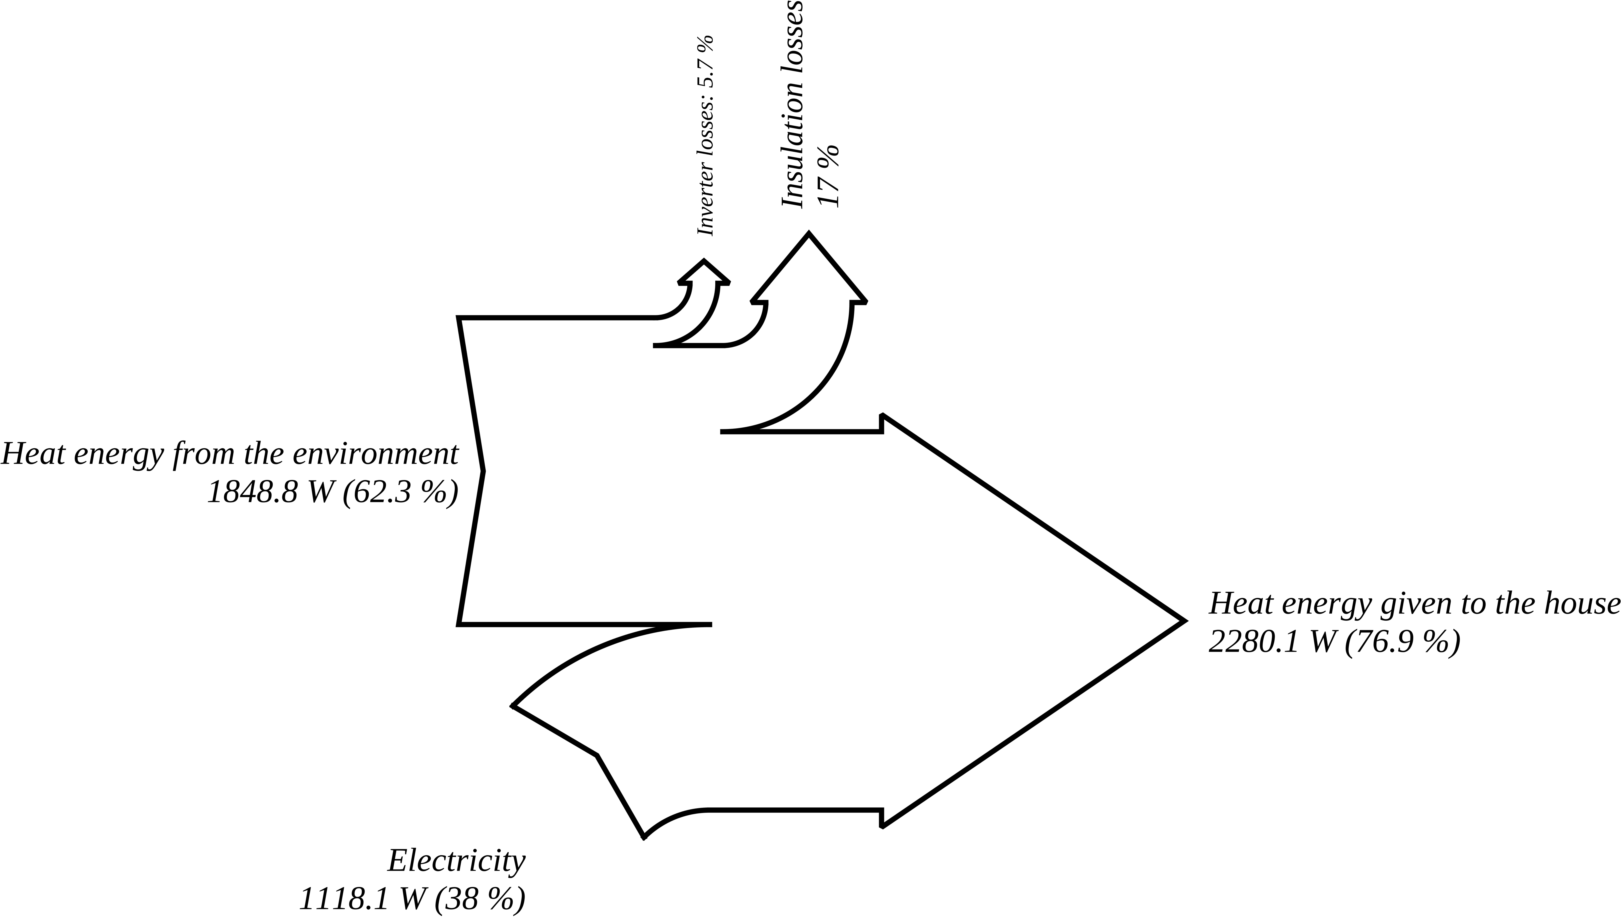
\includegraphics[width=0.7\textwidth]{bwp-energy-sankey-bwp-break}
  \caption{B8.0/W11.0 -- Sankey diagram for heat pump energy balance (internal frontier)}
  \label{fig:bwp-B8.0/W11.0-sankey-energy}
\end{figure}


\begin{figure}[htbp]
  \centering
  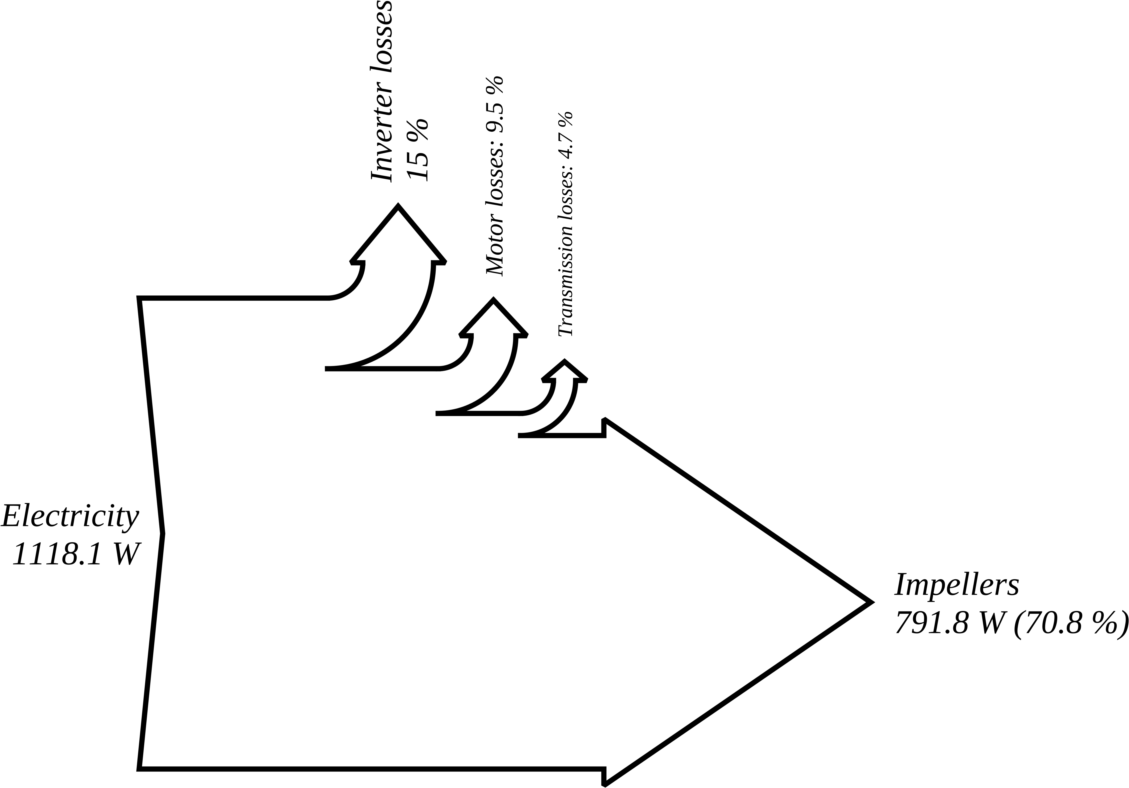
\includegraphics[width=0.7\textwidth]{bwp-energy-sankey-cp-break}
  \caption{B8.0/W11.0 -- Sankey diagram for the compressor unit energy balance}
  \label{fig:bwp-B8.0/W11.0-sankey-cp}
\end{figure}


\begin{figure}[htbp]
  \centering
  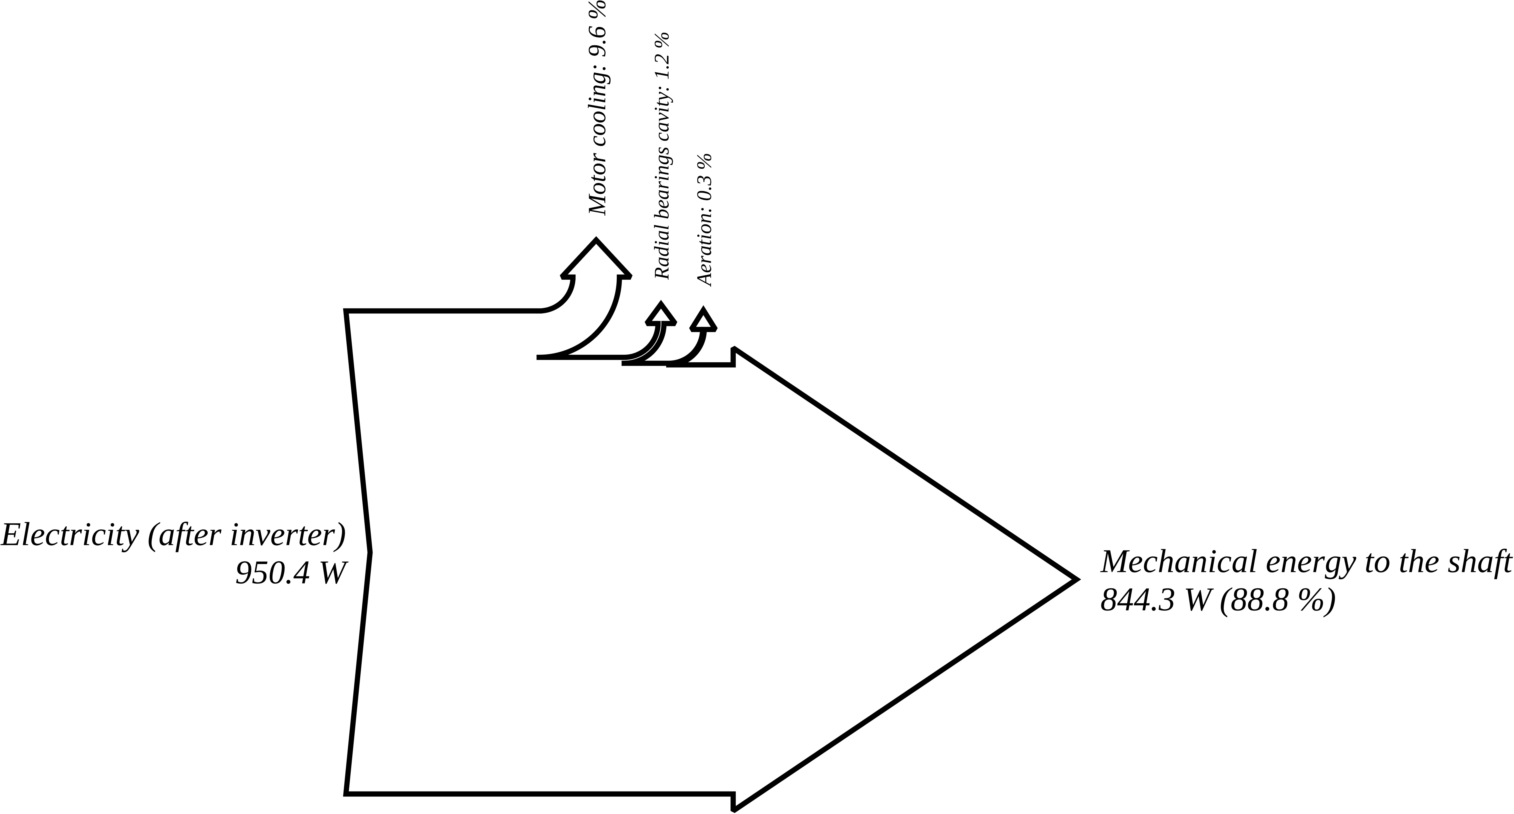
\includegraphics[width=0.7\textwidth]{bwp-energy-sankey-motor-break}
  \caption{B8.0/W11.0 -- Sankey diagram for the motor energy balance}
  \label{fig:bwp-B8.0/W11.0-sankey-motor}
\end{figure}

\begin{table}[htbp]
    \footnotesize
    \begin{center}
    \begin{tabular}{llllll}
\toprule
Name & Value / \% & Name & Value / \% & Name & Value / - \\
\midrule
$\eta_{heatpump}$ & $ \num{7} \pm \num{7} $ & $\eta_{motor}$ & $ \num{88} \pm \num{2} $ & $\epsilon_h$ & $ \num{1.95} \pm \num{1.95} $\\
$\eta_{cp1}$ & $ \num{72} \pm \num{1} $ & $\eta_{cp2}$ &$ \num{26.1} \pm \num{0.5} $ & $\pi_1$ & $ \num{1.64} \pm \num{1.64} $\\
$\eta_{cp1,\,imp}$ & $ \num{73} \pm \num{26} $ & $\eta_{cp2,\,imp}$ & $ \num{75} \pm \num{2} $ & $\pi_2$ & $ \num{1.4032} \pm \num{1e+00} $\\
$\eta_{cd}$ & $ \num{25} \pm \num{25} $ & $\eta_{ev}$ & $ \num{58} \pm \num{20} $ & $\pi_{1,\,theory}$ & $ \num{1.56} \pm \num{1.56} $\\
$\eta_{trans}$ & $ \num{93.78} \pm \num{0.03} $ & $\eta_{sc}$ & N/A & $\pi_{2,\,theory}$ & $ \num{1.3} \pm \num{1.3} $\\
$\eta_{s,\,cp1}$ & $ \num{71} \pm \num{29} $ & $\eta_{s,\,cp2}$ & $ \num{72.8} \pm \num{0.3} $ & $\eta_{motor}$ & $\underline{86.04}$ \%\\
$\eta_{s,\,cp1,\,ext}$ & $ \num{72.6} \pm \num{0.3} $ & $\eta_{s,\,cp2,\,ext}$ & $ \num{72.8} \pm \num{0.3} $ & $\eta_{radial}$ & $ \num{97.71} \pm \num{0.03} $ \%\\
$\eta_{s,\,cp1,\,theory}$ & $ \num{79.0} \pm \num{0.4} $ & $\eta_{s,\,cp2,\,theory}$ & $ \num{72} \pm \num{2} $ & $\eta_{axial}$ & $ \num{95.98} \pm \num{0.03} $ \%\\
\bottomrule
\end{tabular}

  \end{center}
  \caption{B8.0/W11.0 -- Performance indicators}
\end{table}

\begin{figure}[htbp]
  \centering
  \subfloat[Absolute pressures at the bearings cavity]
  {\label{fig:bwp-bearings-P}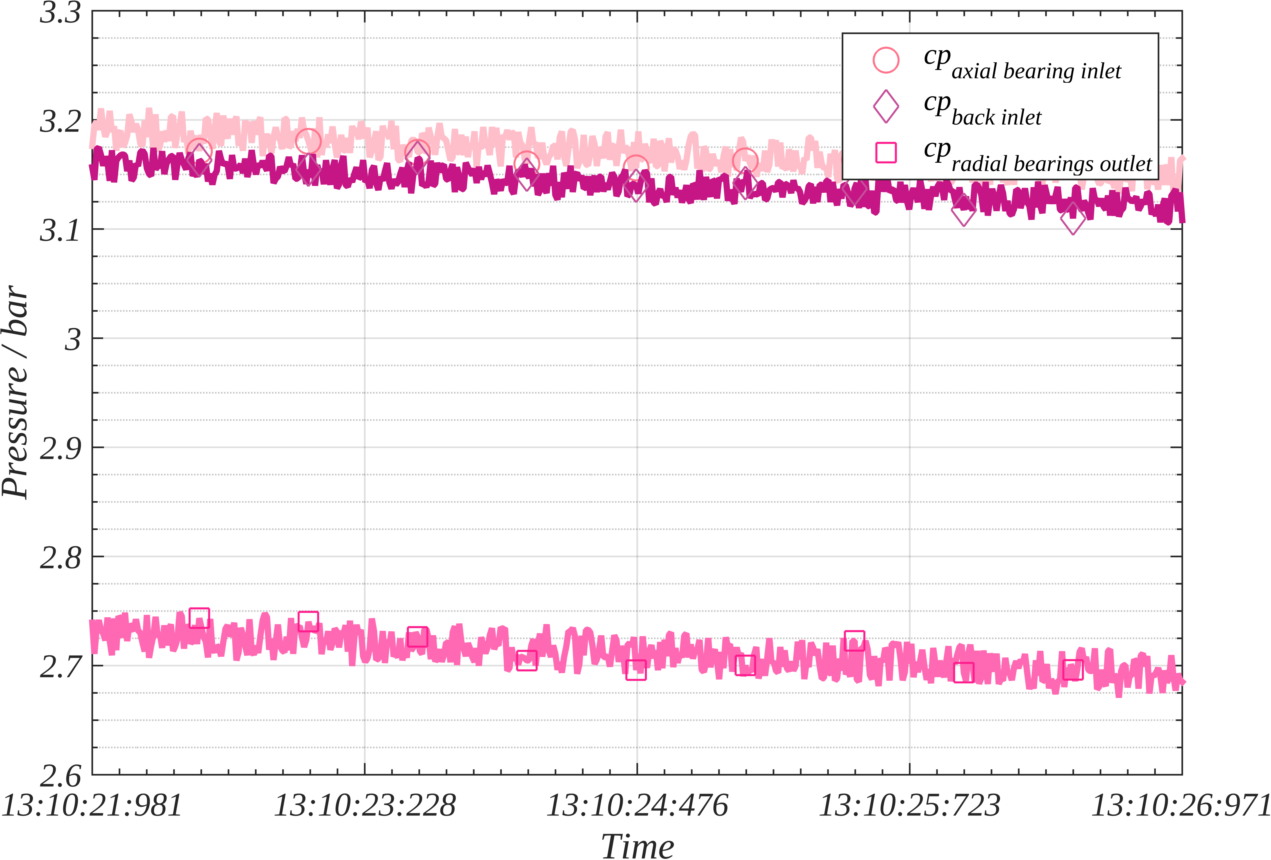
\includegraphics[width=0.45\textwidth]{bwp-bearings-P}}
  \hspace{1em}
  \subfloat[Temperatures at the bearings cavity]
  {\label{fig:bwp-bearings-T}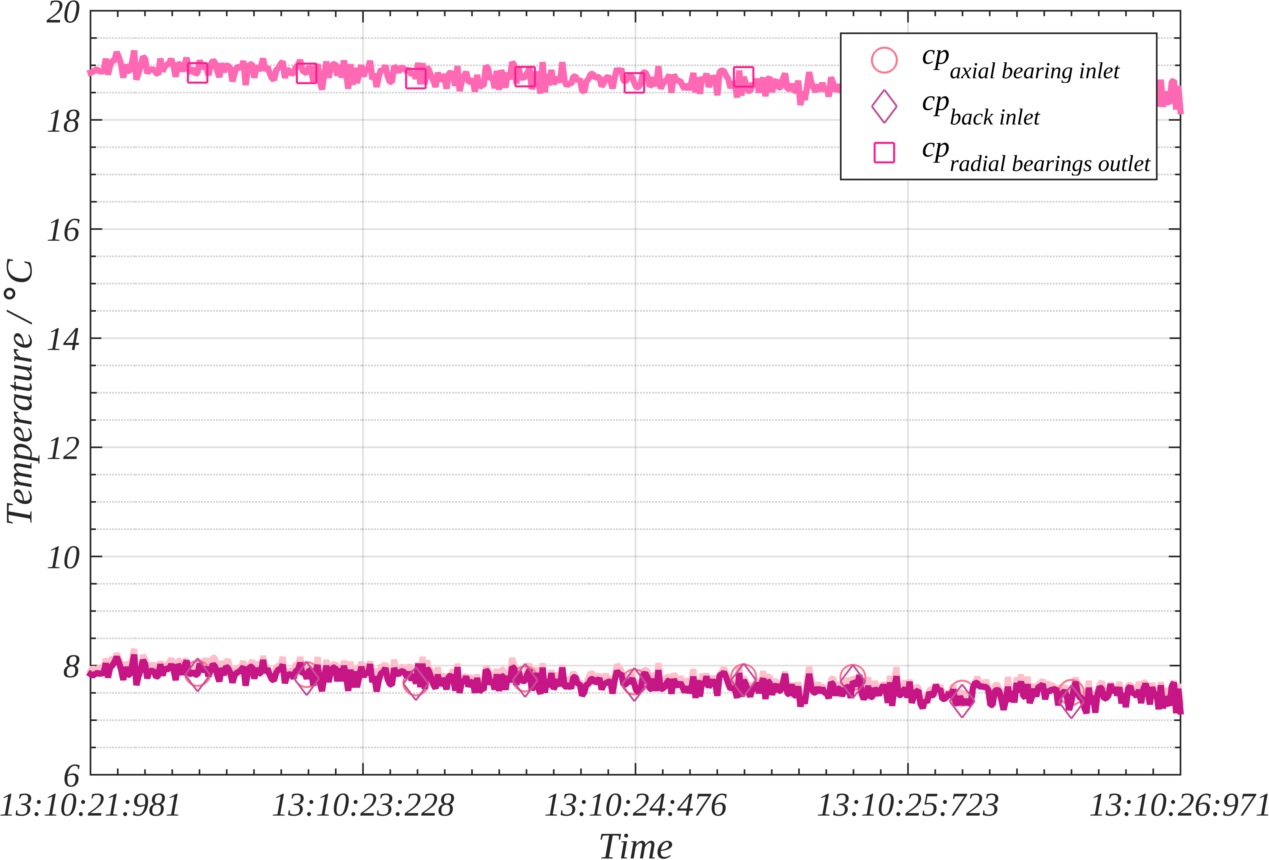
\includegraphics[width=0.45\textwidth]{bwp-bearings-T}}
  \caption[Pressures and temperatures at the bearings cavity when the
  breakdown happened]{Absolute pressures and temperatures at the
    bearings cavity when the breakdown happened}
  \label{fig:bwp-bearings-P-T}
\end{figure}

\begin{figure}[htbp]
  \centering
  \subfloat[Absolute pressures at the compression unit]
  {\label{fig:bwp-cp-P}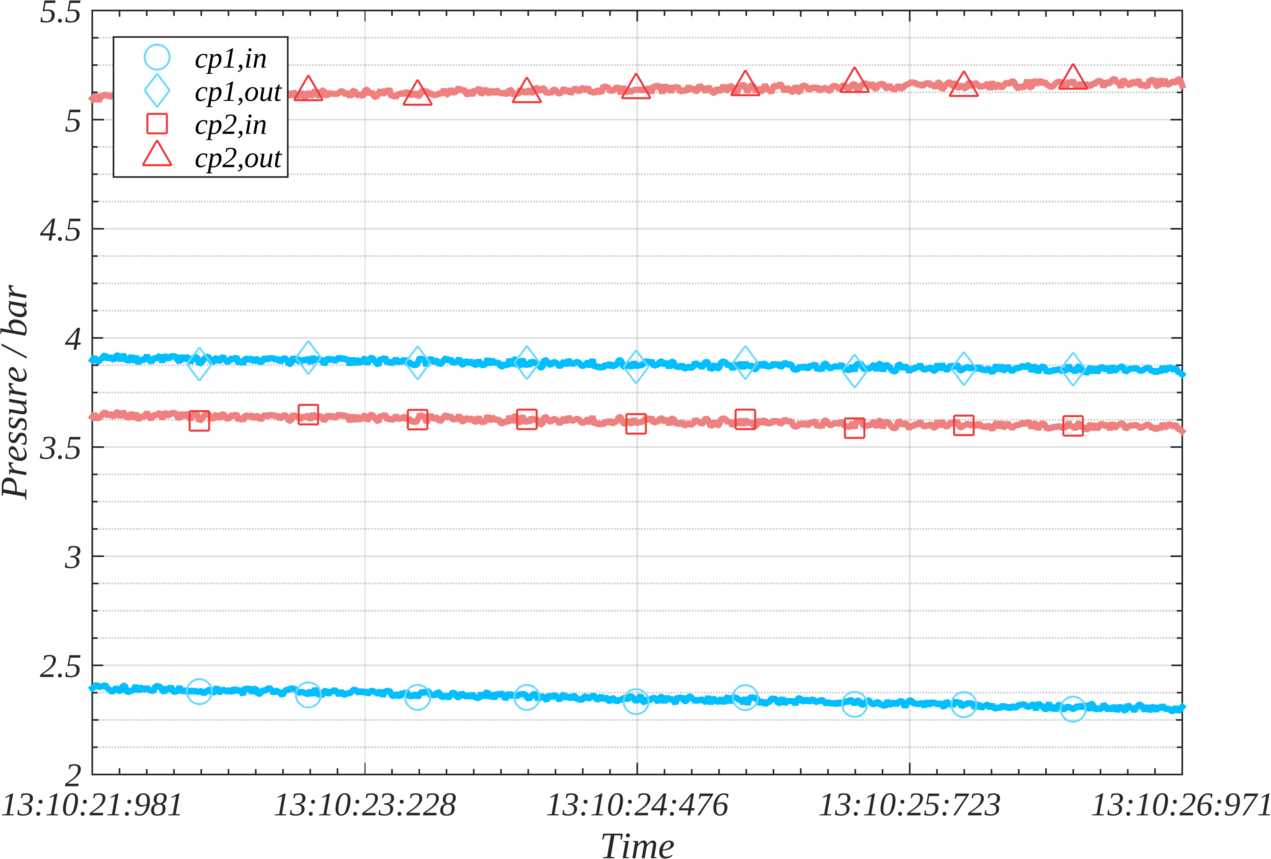
\includegraphics[width=0.45\textwidth]{bwp-cp-P}}
  \hspace{1em}
  \subfloat[Temperatures at the compression unit]
  {\label{fig:bwp-cp-T}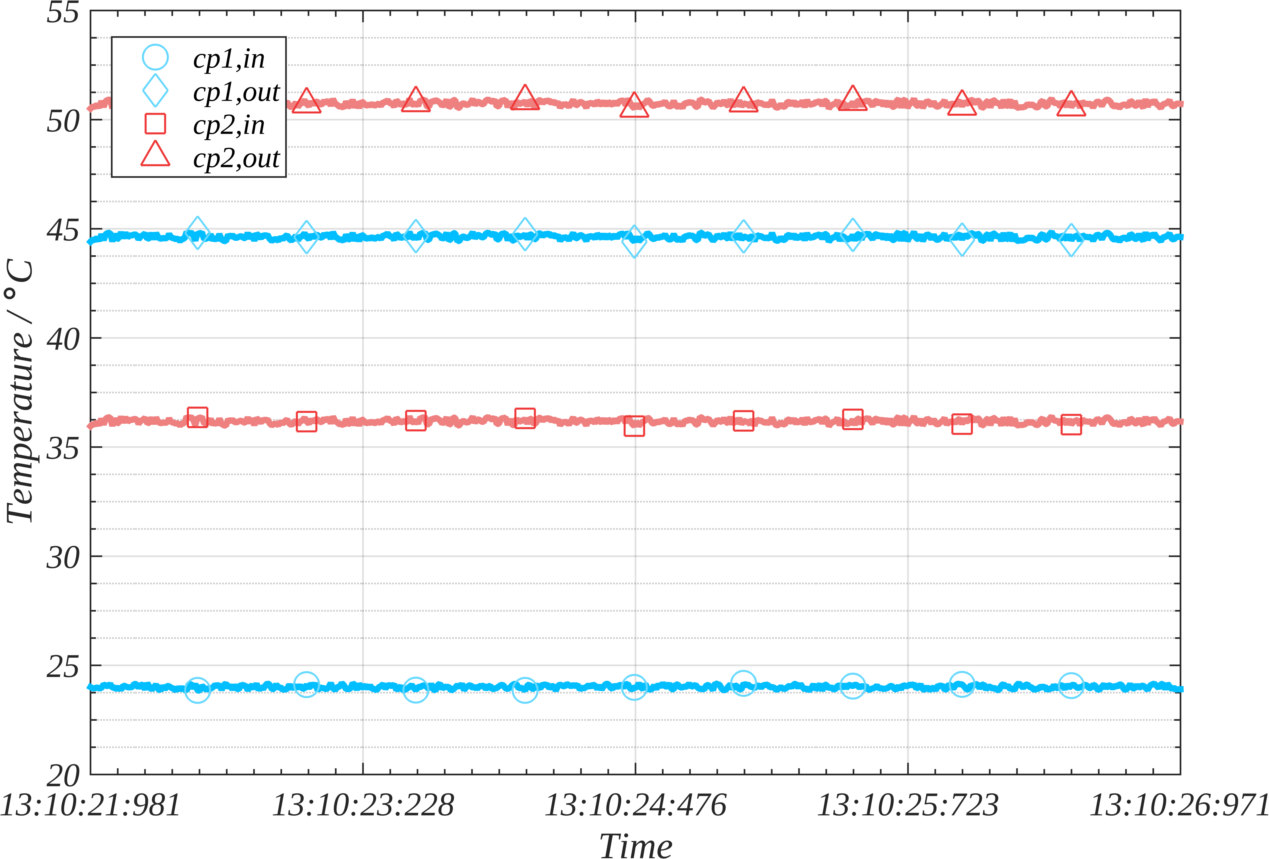
\includegraphics[width=0.45\textwidth]{bwp-cp-T}}
  \caption[Pressures and temperatures at compression unit
  inlets/outlets when the breakdown happened]{Absolute pressures and
    temperatures at compression unit inlets/outlets when the breakdown
    happened}
  \label{fig:bwp-cp-P-T}
\end{figure}

\begin{figure}[htbp]
  \centering
  \subfloat[Power consumption]
  {\label{fig:bwp-cp-P}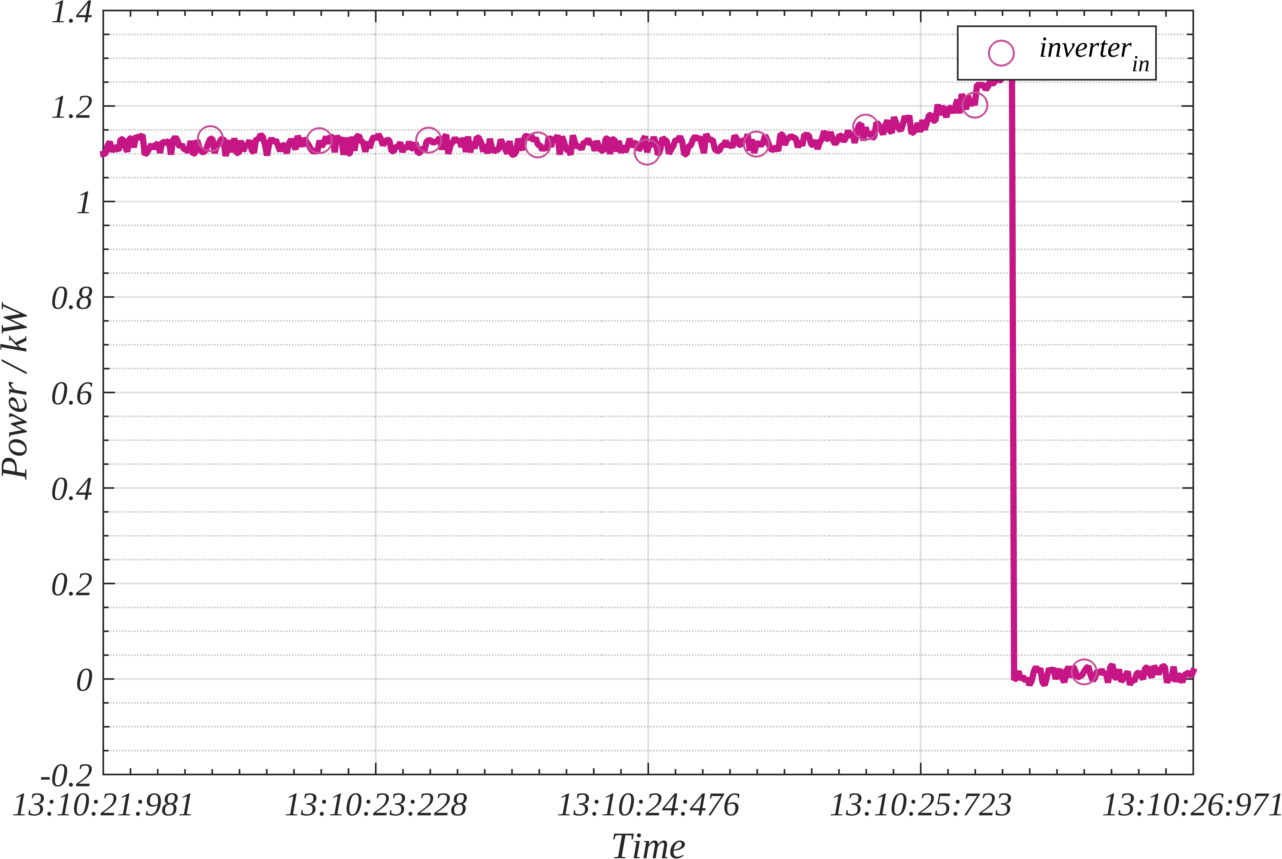
\includegraphics[width=0.45\textwidth]{bwp-power}}
  \hspace{1em}
  \subfloat[Speed]
  {\label{fig:bwp-cp-T}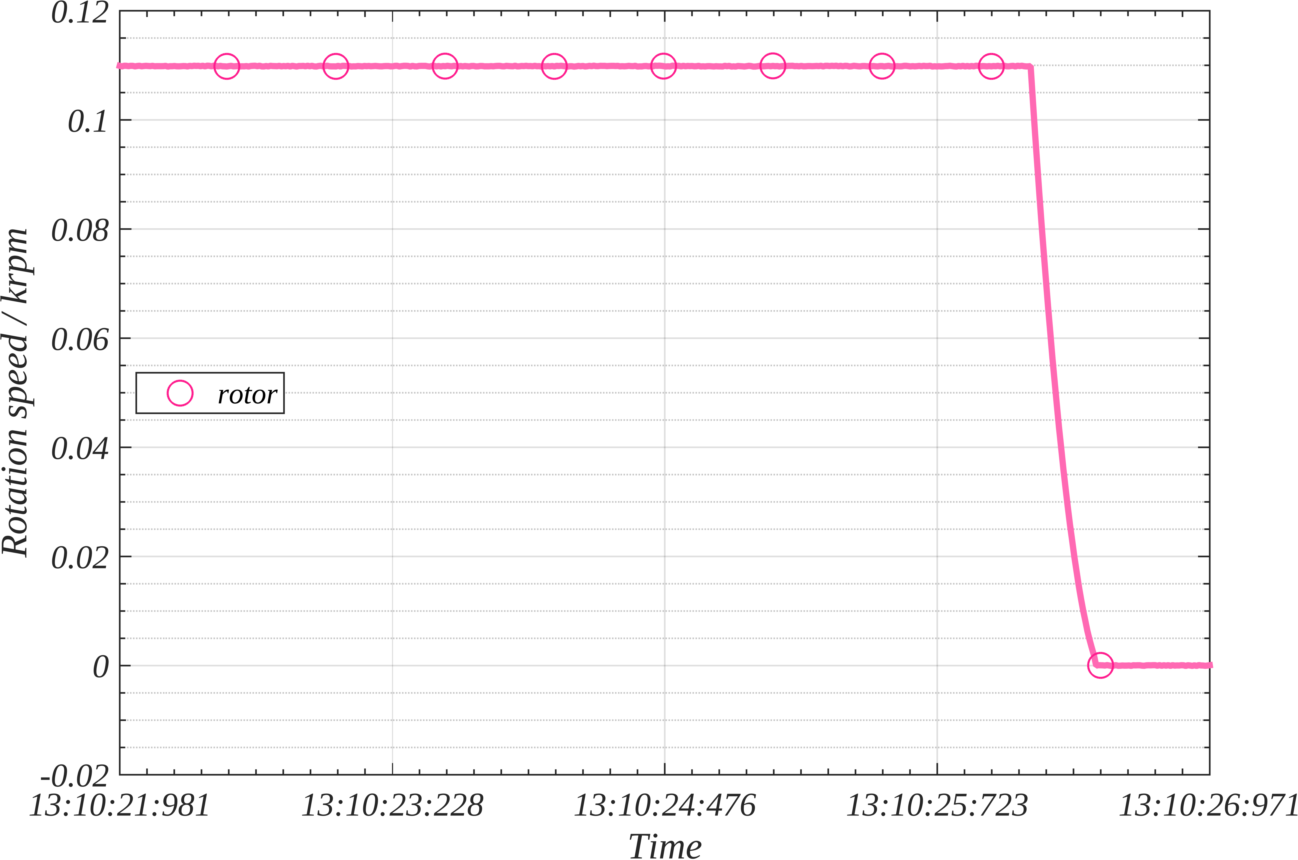
\includegraphics[width=0.45\textwidth]{bwp-speed}}
  \caption{Power comsumption and rotational speed records when the breakdown happened}
  \label{fig:bwp-cp-P-T}
\end{figure}

\FloatBarrier
